

\tikzset{every picture/.style={line width=0.75pt}} %set default line width to 0.75pt

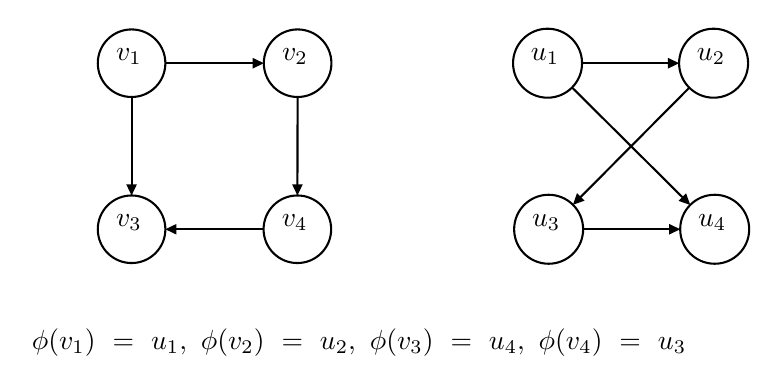
\begin{tikzpicture}[x=0.75pt,y=0.75pt,yscale=-1,xscale=1]
%uncomment if require: \path (0,184); %set diagram left start at 0, and has height of 184


% Text Node
\draw (5,157.4) node [anchor=north west][inner sep=0.75pt]    {$\phi ( v_{1}) \ =\ u_{1} ,\ \phi ( v_{2}) \ =\ u_{2} ,\ \phi ( v_{3}) \ =\ u_{4} ,\ \phi ( v_{4}) \ =\ u_{3}$};
% Text Node
\draw    (335.5, 111) circle [x radius= 16.62, y radius= 16.62]   ;
\draw (326,102.4) node [anchor=north west][inner sep=0.75pt]    {$u_{4}$};
% Text Node
\draw    (255.5, 111) circle [x radius= 16.62, y radius= 16.62]   ;
\draw (246,102.4) node [anchor=north west][inner sep=0.75pt]    {$u_{3}$};
% Text Node
\draw    (54.56, 31) circle [x radius= 16.28, y radius= 16.28]   ;
\draw (45.56,22.4) node [anchor=north west][inner sep=0.75pt]    {$v_{1}$};
% Text Node
\draw    (54.56, 111) circle [x radius= 16.28, y radius= 16.28]   ;
\draw (45.56,102.4) node [anchor=north west][inner sep=0.75pt]    {$v_{3}$};
% Text Node
\draw    (134.56, 31) circle [x radius= 16.28, y radius= 16.28]   ;
\draw (125.56,22.4) node [anchor=north west][inner sep=0.75pt]    {$v_{2}$};
% Text Node
\draw    (134.44, 111) circle [x radius= 16.28, y radius= 16.28]   ;
\draw (125.44,102.4) node [anchor=north west][inner sep=0.75pt]    {$v_{4}$};
% Text Node
\draw    (254.98, 31) circle [x radius= 16.62, y radius= 16.62]   ;
\draw (245.48,22.4) node [anchor=north west][inner sep=0.75pt]    {$u_{1}$};
% Text Node
\draw    (334.98, 31) circle [x radius= 16.62, y radius= 16.62]   ;
\draw (325.48,22.4) node [anchor=north west][inner sep=0.75pt]    {$u_{2}$};
% Connection
\draw    (272.12,111) -- (315.88,111) ;
\draw [shift={(318.88,111)}, rotate = 180] [fill={rgb, 255:red, 0; green, 0; blue, 0 }  ][line width=0.08]  [draw opacity=0] (5.36,-2.57) -- (0,0) -- (5.36,2.57) -- cycle    ;
% Connection
\draw    (54.56,47.28) -- (54.56,91.72) ;
\draw [shift={(54.56,94.72)}, rotate = 270] [fill={rgb, 255:red, 0; green, 0; blue, 0 }  ][line width=0.08]  [draw opacity=0] (5.36,-2.57) -- (0,0) -- (5.36,2.57) -- cycle    ;
% Connection
\draw    (70.84,31) -- (115.28,31) ;
\draw [shift={(118.28,31)}, rotate = 180] [fill={rgb, 255:red, 0; green, 0; blue, 0 }  ][line width=0.08]  [draw opacity=0] (5.36,-2.57) -- (0,0) -- (5.36,2.57) -- cycle    ;
% Connection
\draw    (134.54,47.28) -- (134.47,91.72) ;
\draw [shift={(134.46,94.72)}, rotate = 270.09000000000003] [fill={rgb, 255:red, 0; green, 0; blue, 0 }  ][line width=0.08]  [draw opacity=0] (5.36,-2.57) -- (0,0) -- (5.36,2.57) -- cycle    ;
% Connection
\draw    (118.16,111) -- (73.84,111) ;
\draw [shift={(70.84,111)}, rotate = 360] [fill={rgb, 255:red, 0; green, 0; blue, 0 }  ][line width=0.08]  [draw opacity=0] (5.36,-2.57) -- (0,0) -- (5.36,2.57) -- cycle    ;
% Connection
\draw    (271.6,31) -- (315.36,31) ;
\draw [shift={(318.36,31)}, rotate = 540] [fill={rgb, 255:red, 0; green, 0; blue, 0 }  ][line width=0.08]  [draw opacity=0] (5.36,-2.57) -- (0,0) -- (5.36,2.57) -- cycle    ;
% Connection
\draw    (266.77,42.71) -- (321.58,97.17) ;
\draw [shift={(323.71,99.29)}, rotate = 224.81] [fill={rgb, 255:red, 0; green, 0; blue, 0 }  ][line width=0.08]  [draw opacity=0] (5.36,-2.57) -- (0,0) -- (5.36,2.57) -- cycle    ;
% Connection
\draw    (323.27,42.79) -- (269.33,97.08) ;
\draw [shift={(267.21,99.21)}, rotate = 314.81] [fill={rgb, 255:red, 0; green, 0; blue, 0 }  ][line width=0.08]  [draw opacity=0] (5.36,-2.57) -- (0,0) -- (5.36,2.57) -- cycle    ;

\end{tikzpicture}